\documentclass[tikz,border=10pt]{standalone}
\usepackage{tikz}
\usetikzlibrary{shapes, arrows.meta, positioning, fit, backgrounds}

\begin{document}

\begin{tikzpicture}[
    >=Stealth,
    node distance=0.8cm,
    box/.style={rectangle, draw, rounded corners=3pt, minimum height=0.6cm, minimum width=1.8cm, align=center, font=\sffamily\footnotesize, fill=white},
    formula/.style={rectangle, draw, dashed, fill=yellow!8, align=center, font=\sffamily\footnotesize, inner sep=5pt},
    smallbox/.style={rectangle, draw, minimum height=0.5cm, minimum width=1.2cm, align=center, font=\sffamily\scriptsize, fill=white},
    decision/.style={diamond, draw, fill=orange!10, aspect=2, font=\sffamily\scriptsize, inner sep=2pt}
]

    % === ROW 1: ADVERTISERS ===
    \node (advlabel) [font=\sffamily\footnotesize\bfseries] {Advertisers};
    \node (adv1) [smallbox, right=0.5cm of advlabel, fill=purple!8] {Adv 1};
    \node (adv2) [smallbox, right=0.3cm of adv1, fill=purple!8] {Adv 2};
    \node (advdots) [right=0.2cm of adv2, font=\footnotesize] {$\cdots$};
    \node (advn) [smallbox, right=0.2cm of advdots, fill=purple!8] {Adv $n$};

    % === ROW 2: AUTOBIDDING ===
    \node (autobid) [formula, below=0.8cm of adv2] {
        $B_i = \dfrac{pCVR_i \times Price_i}{ROAS_i} \times Pacing_i$
    };
    \node (autobidlabel) [left=0.3cm of autobid, font=\sffamily\footnotesize\bfseries, text width=1.5cm, align=right] {Auto-\\bidding};

    % === ROW 3: SCORING ===
    \node (quality) [box, below left=1cm and 0.5cm of autobid, fill=blue!8] {Quality\\$Q_i \approx pCTR_i$};
    \node (bid) [box, left=0.8cm of quality, fill=blue!8] {Bid\\$B_i$};
    \node (times) [right=0.3cm of quality, font=\large] {$\times$};
    \node (arrow1) [right=0.3cm of times] {};
    \node (score) [box, right=0.3cm of times, fill=yellow!15] {Score\\$S_i = B_i \times Q_i$};

    % === ROW 4: AUCTION ===
    \node (auction) [box, below=1cm of score, fill=gray!15, minimum width=2.5cm] {Auction: Rank by $S_i$};

    % === ROW 5: SLOTS ===
    \node (slot1) [smallbox, below left=0.8cm and 1cm of auction, fill=green!20] {Rank 1};
    \node (slot2) [smallbox, right=0.3cm of slot1, fill=green!12] {Rank 2};
    \node (slot3) [smallbox, right=0.3cm of slot2, fill=green!6] {Rank 3};
    \node (slotdots) [right=0.2cm of slot3, font=\footnotesize] {$\cdots$};

    % === USER FUNNEL (right side) ===
    \node (user) [box, right=3cm of autobid, fill=gray!10] {User Query};
    \node (impress) [box, below=0.8cm of user] {Impression};
    \node (click) [decision, below=0.6cm of impress] {Click?};
    \node (purchase) [decision, below=0.6cm of click] {Buy?};
    \node (revenue) [box, below=0.6cm of purchase, fill=green!20] {Revenue};

    % === EDGES: AUCTION FLOW ===
    \draw[->, thick] (adv1.south) -- ++(0,-0.3) -| (autobid.north);
    \draw[->, thick] (adv2.south) -- (autobid.north);
    \draw[->, thick] (advn.south) -- ++(0,-0.3) -| (autobid.north);

    \draw[->, thick] (autobid.south) -- ++(0,-0.3) -| (bid.north);
    \draw[->, thick] (autobid.south) -- ++(0,-0.3) -| (quality.north);

    \draw[->, thick] (bid.east) -- ++(0.2,0);
    \draw[->, thick] (score.south) -- (auction.north);

    \draw[->, thick] (auction.south) -- ++(0,-0.3) -| (slot1.north);
    \draw[->, thick] (auction.south) -- ++(0,-0.3) -| (slot2.north);
    \draw[->, thick] (auction.south) -- ++(0,-0.3) -| (slot3.north);

    % === EDGES: USER FUNNEL ===
    \draw[->, thick] (user) -- (impress);
    \draw[->, thick] (impress) -- (click);
    \draw[->, thick] (click) -- node[right, font=\scriptsize] {Y} (purchase);
    \draw[->, thick] (purchase) -- node[right, font=\scriptsize] {Y} (revenue);
    \draw[->] (click.west) -- ++(-0.4,0) node[left, font=\scriptsize] {N};
    \draw[->] (purchase.west) -- ++(-0.4,0) node[left, font=\scriptsize] {N};

    % === CROSS CONNECTION ===
    \draw[->, thick, blue!60] (slot2.east) -- ++(0.5,0) |- (impress.west);
    \draw[->, thick, blue!60] (user.west) -- ++(-0.5,0) |- (auction.east);

    % === FEEDBACK ===
    \draw[->, dashed, gray] (click.east) -- ++(0.5,0) |- ++(0,3.5) -| node[pos=0.2, above, font=\scriptsize\sffamily, gray] {feedback} (quality.north);

    % === LABELS ===
    \begin{scope}[on background layer]
        \node[fit=(bid)(quality)(score)(auction)(slot1)(slotdots),
              draw=purple!30, fill=purple!3, rounded corners, inner sep=10pt] (abox) {};
        \node[fit=(user)(impress)(click)(purchase)(revenue),
              draw=blue!30, fill=blue!3, rounded corners, inner sep=10pt] (ubox) {};
    \end{scope}

    \node[above=0.1cm of abox.north, font=\sffamily\bfseries\footnotesize, purple!70] {Auction Mechanics};
    \node[above=0.1cm of ubox.north, font=\sffamily\bfseries\footnotesize, blue!70] {User Funnel};

\end{tikzpicture}

\end{document}
